\section{Calculating $\pi$}

\epigraph{\emph{The best programs are written so that computing machines
    can perform them quickly and so that human beings can understand
    them clearly. A programmer is ideally an essayist who works with
    traditional aesthetic and literary forms as well as mathematical
concepts, to communicate the way that an algorithm works and to convince
a reader that the results will be correct.}}{---Donald Knuth}\noindent

Why, you might ask, do we need to calculate $\pi$? In practice, we do
not: it is available as part of the of the \texttt{<math.h>} library as
\texttt{M\_PI}, since we do need it for all manner of scientific and
engineering calculations. The area of a circle is $\pi r^2$ and the
volume of a sphere is $\frac{4}{3} \pi r^3.$  The cosmological constant
is $$\Lambda = \frac{8 \pi G}{3 c^2} \rho.$$  Heisenberg's uncertainty
principle is given by $$\Delta x \Delta p \ge \frac{h}{4 \pi}.$$
Einstein's general relativity field equation is $$R_{\mu\nu} -
\frac{1}{2}g_{\mu\nu} +\Lambda g_{\mu\nu} = \frac{8 \pi G}{c^4}
T_{\mu\nu},$$ and so forth. No matter where you look, $\pi$ is pervasive
in the physical world.

So why do we calculate it? Well, suppose the person who typed up the
\texttt{<math.h>} file made a mistake.  Or, perhaps you need more
accuracy than is normally provided. But ultimately, most people do it
for the sheer fun of it. Computations such as finding the most digits of
$\pi$ fall into the area of experimental mathematics.

Experimental mathematics is an approach to mathematics in which
computation is used to investigate mathematical objects and identify
properties and patterns. It has been defined in a discussion by
J.\xspace Borwein, P.\xspace Borwein, R.\xspace Girgensohn and S.\xspace
Parnes as ``that branch of mathematics that concerns itself ultimately
with the codification and transmission of insights within the
mathematical community through the use of experimental (in either the
Galilean, Baconian, Aristotelian or Kantian sense) exploration of
conjectures and more informal beliefs and a careful analysis of the data
acquired in this pursuit.''

In the subsequent sections, we will present a number of functions $p$
of $n$ that are series that can be used to approximate $\pi$. In each of
these formul\ae\xspace there is a $p(n)$ where the limit
$$\lim_{n\rightarrow\infty} p(n) = \pi.$$ We know, both through
experiment (which usually comes first) and mathematical proof, that
these do result in $\pi$. The question then is: Which of these compute
it most efficiently? Efficiency in this case is measured in the
\emph{number of terms} (or factors, in the case of Wallis and Vi\`{e}te).

\subsection{The Leibniz Formula}

The Leibniz formula for $\pi$ (Gottfried Wilhelm von Leibniz, 1646--1716), given by
$$
p(n)=4 \sum _{k=0}^n \frac{(-1)^k}{2 k+1} = 4 \left ( 1 - \frac{1}{3} +
\frac{1}{5} - \frac{1}{7} + \frac{1}{9} - \cdots\right ) =
\left((-1)^n
   H_{\frac{n}{2}+\frac{1}{4}}-H_{\frac{n}{2}-\frac{1}{4}}\right)+\pi
$$
converges \emph{extremely slowly}, since the \emph{error term} involves \emph{harmonic numbers}, and consequently is not reasonable
for calculation. It is no more than the Taylor series expansion of
$\tan^{-1} x$ with $x=1$.

\begin{figure}[p]
  \centerline{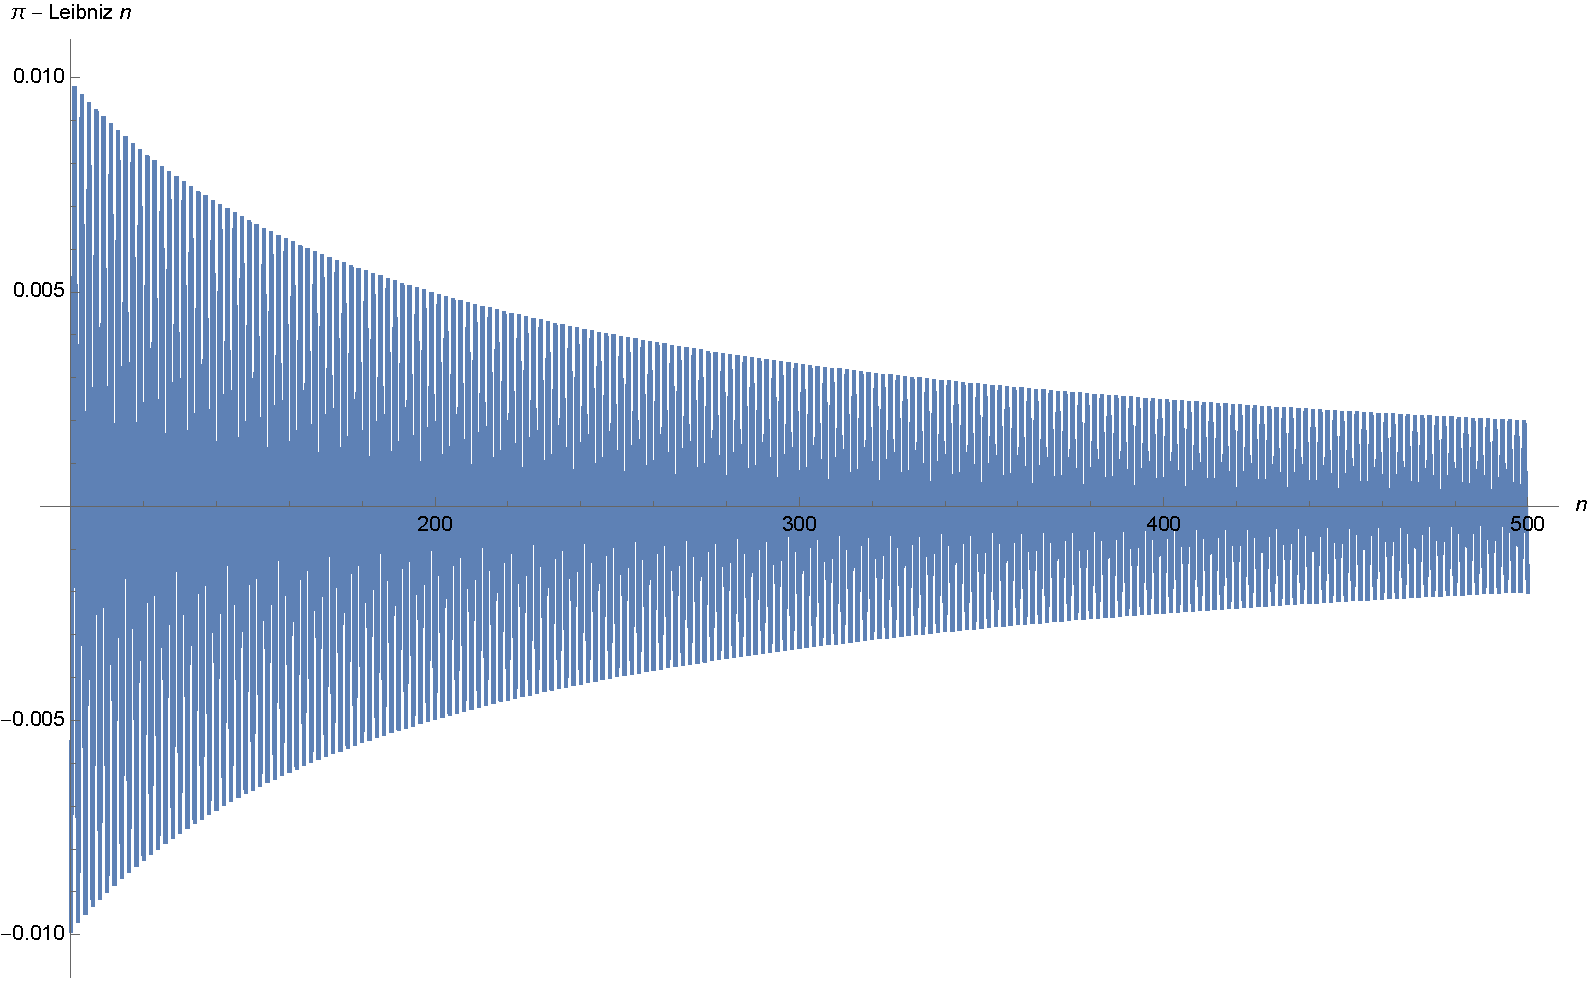
\includegraphics[width=0.75\textwidth]{figures/Leibniz.pdf}}
  \caption{Leibniz sequence $4 \sum _{k=0}^n \frac{(-1)^k}{2 k+1}$}
\end{figure}

\subsection{The Madhava Series}

The Madhava series (M\={a}dhava of Sangamagr\={a}ma, c.\xspace 1340 --
c.\xspace 1425) is also related to $\tan^{-1} x$,
$$
\sum_{k=0}^\infty \frac{(-3)^{-k}}{2 k+1} =\sqrt{3} \tan^{-1}
\frac{1}{\sqrt{3}} = \frac{\pi}{\sqrt{12}}
$$
but it gives us a more rapidly converging series, given by:
$$
p(n)=\sqrt{12} \sum _{k=0}^n \frac{(-3)^{-k}}{2 k+1} =
\sqrt{12} \left [ \frac{1}{2} 3^{-n-1} \left((-1)^n \Phi \left(-\frac{1}{3},1,n+\frac{3}{2}\right)+\pi
   3^{n+\frac{1}{2}}\right) \right ].
$$
Which leaves us with the problem of calculating $\sqrt{12}$. You may be
thinking: ``Can't I just use the library?'' The answer, of course, is
\emph{no}, you will need to compute $\sqrt{12}$ on your own.
Do you need to worry about $\Phi$? No, you just need to understand that in the limit,
the $\Phi$ term (called the \emph{Lerch transcendent})
 goes to \emph{zero} and that the remaining term
$$
\frac{\pi}{2} 3^{-n-1} 3^{n+\frac{1}{2}} = \frac{\pi}{2 \sqrt{3}} = \frac{\pi}{\sqrt{12}}.
$$

\begin{figure}[p]
  \centerline{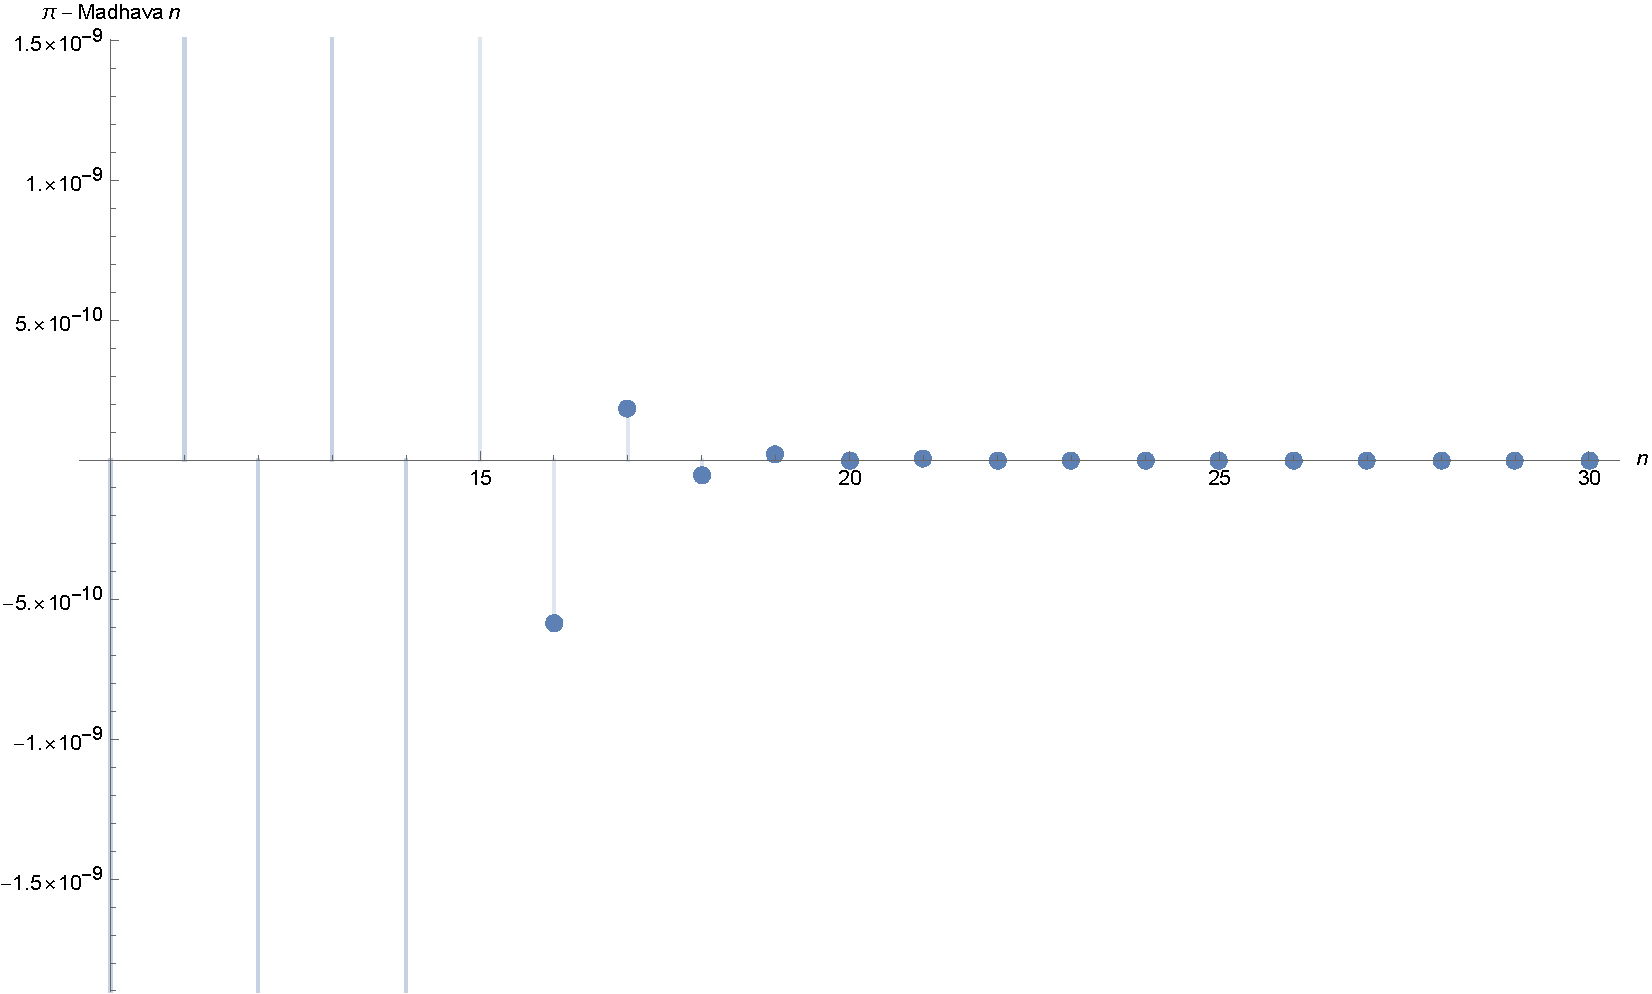
\includegraphics[width=0.75\textwidth]{figures/Madhava.pdf}}
  \caption{Madhava sequence $\sqrt{12} \sum _{k=0}^n \frac{(-3)^{-k}}{2 k+1}$}
\end{figure}

\begin{figure}[p]
  \centerline{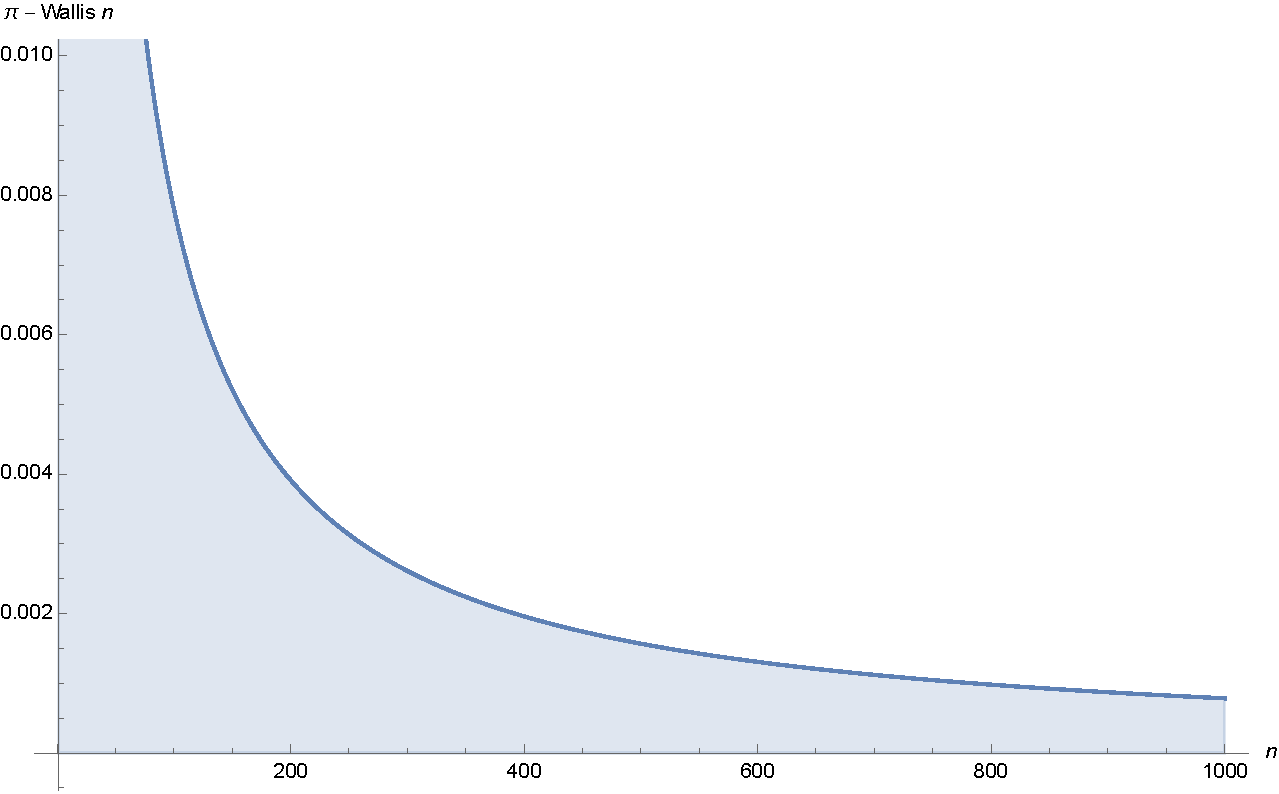
\includegraphics[width=0.75\textwidth]{figures/Wallis.pdf}}
  \caption{Wallis sequence $2 \prod _{k=1}^n \frac{4 k^2}{4 k^2-1}$}
\end{figure}

\subsection{The Wallis Series}

John Wallis (1616--1703) was an English clergyman and mathematician who
is given partial credit for the development of infinitesimal calculus.
He gave us a series that is purely multiplicative (instead of terms, we
have factors):
$$
p(n)=2 \prod _{k=1}^n \frac{4 k^2}{4 k^2-1} = \frac{\pi  \Gamma (n+1)^2}{\Gamma \left(n+\frac{1}{2}\right) \Gamma
   \left(n+\frac{3}{2}\right)}.
$$
It is easy to calculate, but how rapidly does it converge? What is this $\Gamma$ function?
Do we need to compute it?
How do we know this converges to $\pi$?
Let's factor out $\pi$, then take the limit and note that
$$
\underset{n\to \infty }{\text{lim}}\frac{\Gamma (1+n)^2}{\Gamma
   \left(\frac{1}{2}+n\right) \Gamma \left(\frac{3}{2}+n\right)} = 1.
$$
This tells us that as you compute more terms, you get closer to the true value of $\pi$.

\subsection{Euler's Solution}

The Basel problem is a problem in mathematical analysis with relevance
to number theory, first posed by Pietro Mengoli in 1650 and solved by
Leonhard Euler in 1734.  The Basel problem asks for the precise
summation of the reciprocals of the squares of the natural numbers,
\emph{i.e.}\xspace the sum of the infinite series
$$\sum_{k=1}^\infty
\frac{1}{k^2} = \frac{1}{1^2} + \frac{1}{2^2} + \frac{1}{3^2} + \cdots = H_{\infty }^{(2)},$$
which again involves harmonic numbers.
Euler's solution showed that the solution is ${\pi^2}/6$, but his method
gave us this series: $$p(n)=\sqrt{6 \sum_{k=1}^n \frac{1}{k^2}}$$ which
also requires us to calculate the square root, of this case an unknown
(until we calculate it) number.

\begin{figure}
  \centerline{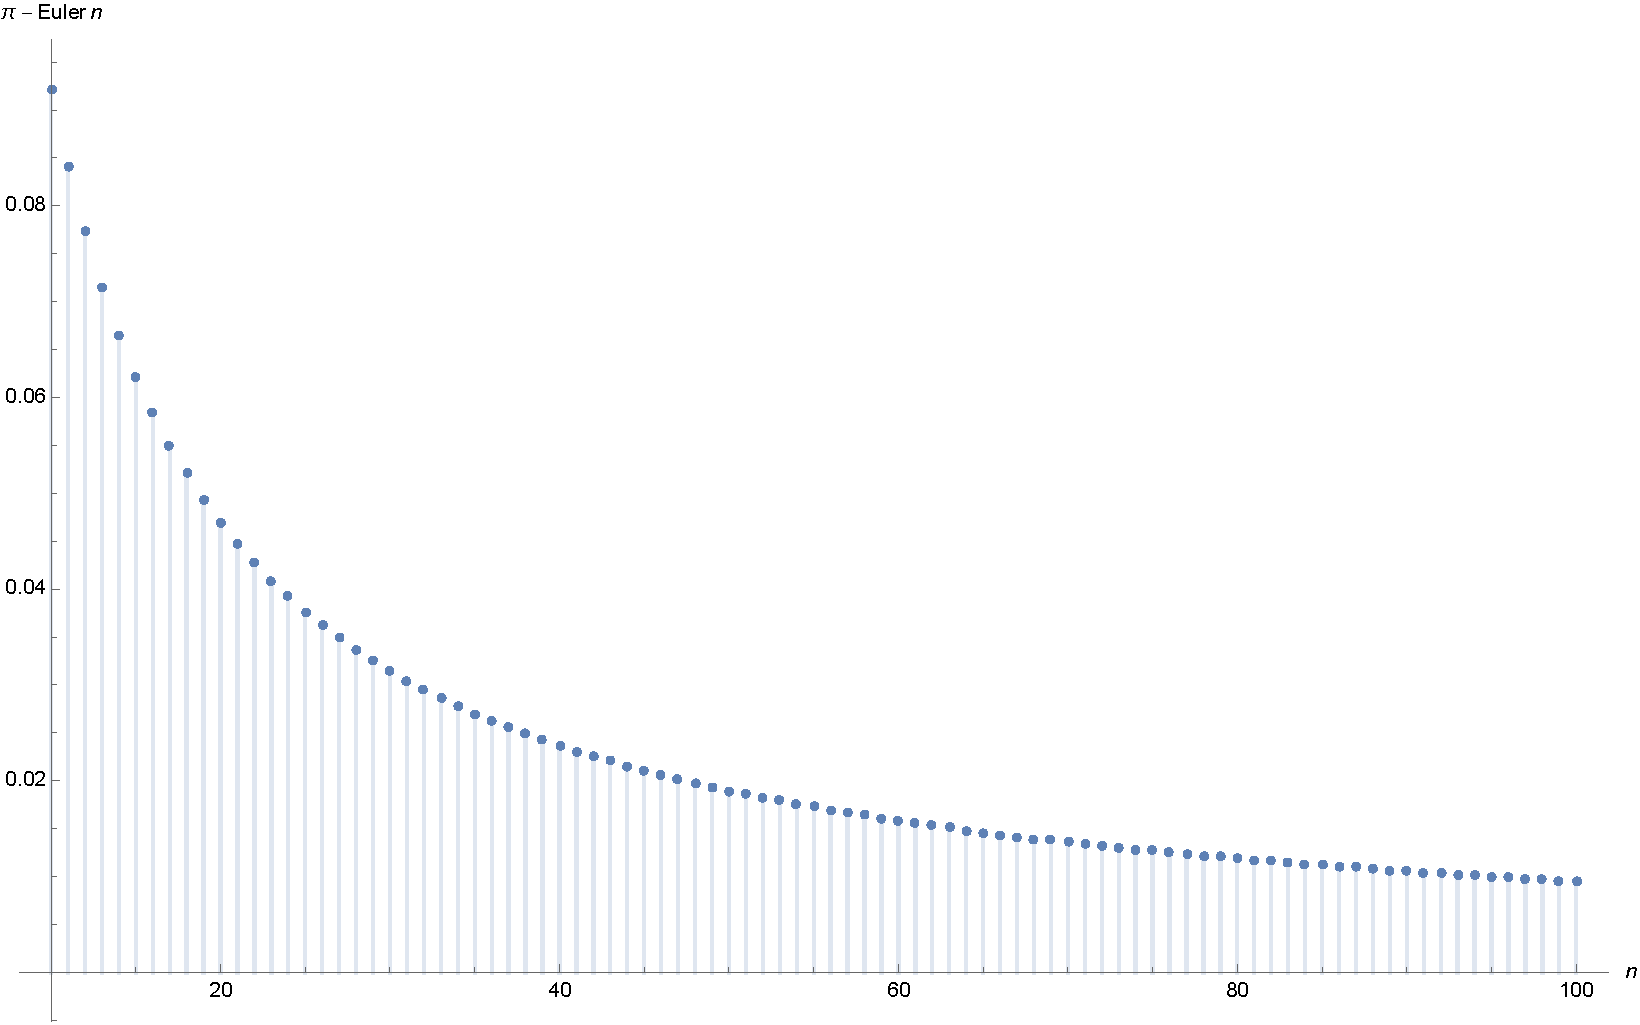
\includegraphics[width=0.75\textwidth]{figures/Euler.pdf}}
  \caption{Euler sequence $\sqrt{6 \sum _{k=1}^n \frac{1}{k^2}}$}
\end{figure}

\subsection{The Bailey-Borwein-Plouffe Formula}

The Bailey-Borwein-Plouffe formula (BBP formula) is a formula for $\pi$.
It was discovered in 1995 by Simon Plouffe and is named after the
authors of the article in which it was published, David H.\xspace
Bailey, Peter Borwein, and Plouffe. The formula that they discovered is
remarkably simple:
$$
p(n)=\sum _{k=0}^n {16^{-k}}\Biggl ( {\frac{4}{8 k+1}-\frac{2}{8
  k+4}-\frac{1}{8 k+5}-\frac{1}{8 k+6}} \Biggl ) .
$$
And if you desire to reduce it to the least number of multiplications,
you can rewrite it in \emph{Horner normal form}:
$$
p(n)=\sum _{k=0}^n {16^{-k}}\times \frac{ (k (120 k+151)+47)}{k (k (k
(512 k+1024)+712)+194)+15} .
$$

\subsection{Vi\`{e}te's Formula}

Named after Fran\c{c}ois Vi\`{e}te, Vi\`{e}te's formula is a infinite
product of nested radicals that can be used for calculations of $\pi$,
though it should be noted that methods found before this specific
formula are known to produce greater accuracy.

Vi\`{e}te's formula can be written as follows:
\[
  \frac{2}{\pi} = \frac{\sqrt{2}}{2} \times \frac{\sqrt{2 +
  \sqrt{2}}}{2} \times \frac{\sqrt{2 + \sqrt{2 + \sqrt{2}}}}{2} \cdots
\]

Or more simply,
\[
  \frac{2}{\pi} = \prod_{k=1}^{\infty} \frac{a_k}{2}
\]
where $a_1 = \sqrt{2}$ and $a_k = \sqrt{2 + a_{k-1}}$ for all $k > 1$.


\subsection{Fastest Series}

Perhaps the most interesting is the series given by Srinivasa Ramanujan
(1887--1920)
$$
\frac{1}{\pi}=
\sum_{k=0}^\infty
\frac{2 \sqrt{2}}{9801} \times
\frac{(4k)!  (1101 + 26390 k)}{(k!)^4 396^{4k}}
$$
which was later extended by the Chudnovsky brothers (whose lives seem to
be centered around the calculation of $\pi$) to the series:
$$
\frac{1}{\pi} = 12 \sum_{k=0}^\infty \frac{(-1)^k (6k)! (13591409 +
545140134 k)}{(3k)! (k!)^3 640320^{3k + 3/2}} .
$$
If you can find no particular significance in the constants in
Ramanujan's formula, then perhaps we should give up any hope of
understanding the Chudnovsky's!

Ultimately, what we have learned is this: we cannot know $\pi$ exactly,
but we know relations that involve $\pi$ that we can approximate using a
series. The question then becomes: Which series converges to $\pi$ most
rapidly?
